\section{Problem analysis}
\ninanotes{
\begin{itemize}
\item Coarse problem analysis Describing the problem and goals in more
detail, briefly analysing the challenges, pointing out possible solutions.
\item Problem specification and analysis Detailed specification of the
problem (and goals). This might need to introduce new notation in order
to arrive at a precise description. If relevant, make state-of-the-art
solutions precise and compare.
\item Goals and success criteria Describe the goals and when a goal is
reached.
\end{itemize}
}

In this chapter I will go through the main difficulties in coming up with a good solution for Hanabi. Firstly I will go through hardware constraints, then I will motivate my overall solution using dynamic epistemic logic (DEL) and finally I will analyse some lower bounds on time and space this solution would lead to.

\subsection{Hardware and time constraints}
In order to run the self-play of the agents I will have to pick a platform to work on.
The setup I am gonna run the self-play of the agents on is utilizes an Intel® Core™ i7-10875H Processor, with 8 cores and 16 GB of ram. There are also 34GB of swap memory. So there is about 50 GB of memory as an constraint.
In regards to time constraint I want to make have that each agent does not spent much more time than a real-time player. A couple of minutes at most - but this goal is less important, but mostly there to secure that it is actually testable.
The chosen setup and time and memory constraints is mainly due to that is the computer I got, and I now I can iterate fast over a setup I have full control over.


\subsection{A motivation for the solution: Three wise men puzzle}\label{sec:motivation}
In order to motivate my approach to the problem, namely multi-modal logic. 
I will take the example of the three wise men problem.
There are three wise men, each standing in a row, enumarated 1 through 3. 
Then a king, who has 3 red hats and 2 white hats puts a hat on each of the three wise men in such a way that each person does not know the color of the hat on their head. 
Then the king asks the first wise man whether he knows the color of their own hat, where the answer could either be "I don't know" or "I know". 
He then asks the same of the second, then the third.

Let us say that the actual case is RRR i.e. wise man 1, 2 and 3 has a red hat on their head.
In that case wise man 1 will answer: I don't know, the second wise man will answer: I don't know, but the third wise man will answer: I know, how so?

Trying to see the problem from the third wise man's perspective I have illustrated a model at Figure \ref{fig:twm-round-0}. It is based on \KTfourfiveN in \cite{HuthAndRyan2004KT45n}, but breaks with convention used by them in the following way:
The model is strictly from the perspective of wise man 3. So for each possible world of wise man 3, we "fix" this world and then imagine what the other wise men could think was possible based on this. An edge with label x means that wise man x knows this is possible, based on the fixed world of wise man 3.

\begin{figure}
	\begin{minipage}[c]{3cm}
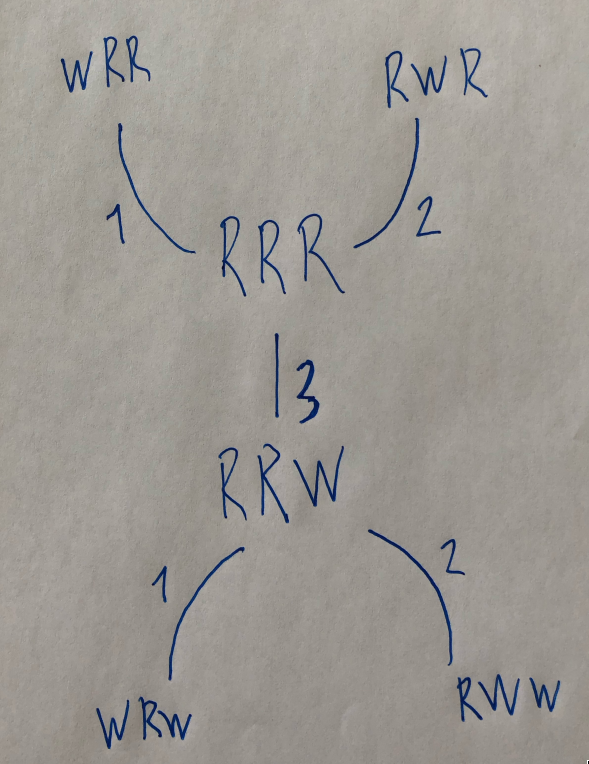
\includegraphics[width=4cm]{images/three_wise_men_round_0.png}
	\caption{The initial model for the third wise man, with no other information than what he can see}

	\label{fig:twm-round-0}
\end{minipage}
\hfill
	\begin{minipage}[c]{3cm}
	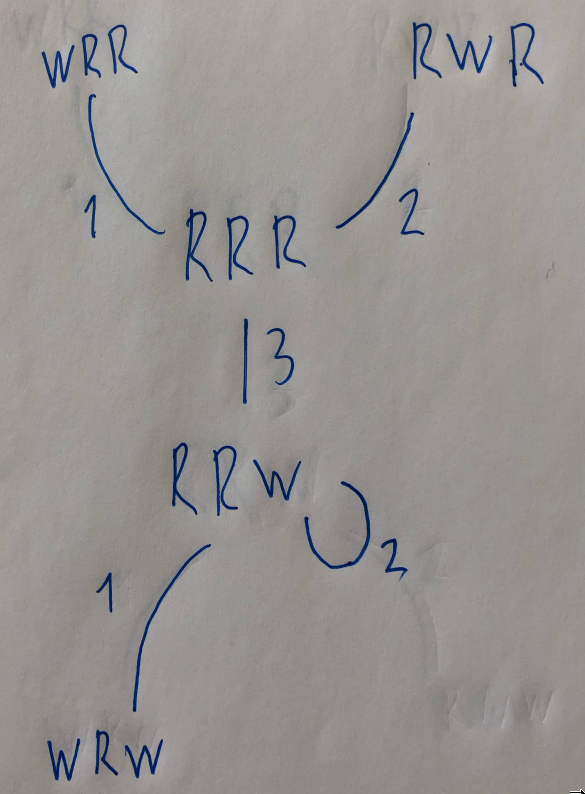
\includegraphics[width=4cm]{images/three_wise_men_round_1.png}
	\caption{The model for the third wise man, after wise man 1 has said "I don't know"}

	\label{fig:twm-round-1}
\end{minipage}
\hfill
	\begin{minipage}[c]{3cm}
	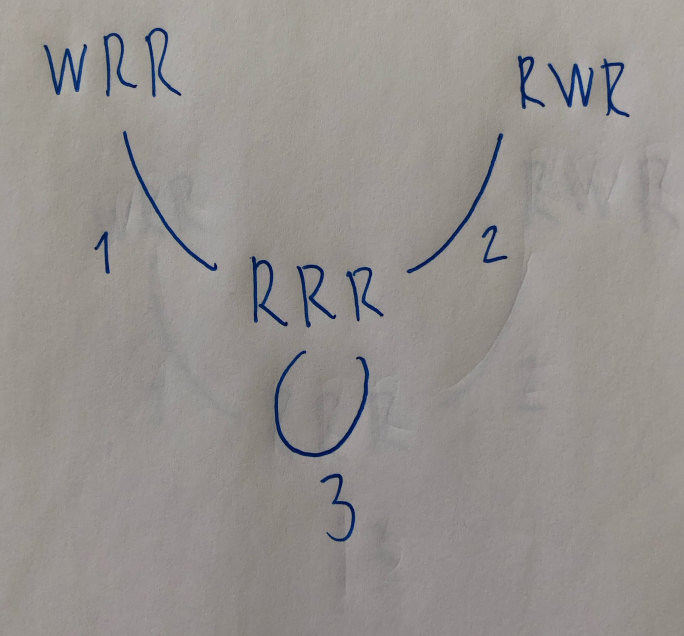
\includegraphics[width=4cm]{images/three_wise_men_round_2.png}
	\caption{The model for the third wise man, after both wise man 1 and two have said "I don't know", in succession.}

	\label{fig:twm-round-2}
\end{minipage}
\end{figure}



Figure \ref{fig:twm-round-0} is the model for the initial configuration. This means that wise man 3 does not know whether he has a red hat or a white hat. And for each of these scenarios he can imagine that 2 cannot know either, and neither can 1. I will refer to scenarios that are fixed from a particular player's POV for \emph{fixed scenarios}. So here the fixed scenarios are RRR and RRW with respect to wise man 3's model.

When 1 states "he does not know" then that has to be equivalent to "not RWW is the case". This means that three can safely eliminate this state, as something 2 would imagine, given that this was a public announcement. This results in the updated model in Figure \ref{fig:twm-round-1}.


After 2 answers "I don't know", wise man 3 can deduce that the case was not RRW, since if it was the case, then 2 would have seen 1:R and 3:W and know that RRW was the only scenario in which this was possible, and hence would answer "I know". Which means that the final model that wise man three has is the one on Figure \ref{fig:twm-round-2}, for which the wise man 3 will know with certainty that the only scenario which is possible is RRR.


\subsection{Description of how modal logic is applied} \label{sec:description-of-how-modal-logic-is_applied}
Without worrying too much about the combinatorial explosion (more on that later), we can apply the principles described in chapter \ref{sec:motivation} to Hanabi. 

So analogously instead of looking at a world as a ordered set of hats, we look at a world as an ordered set of hands. And likewise we can have multiple \emph{fixed scenarios} with respect to the model of the player and imagine what the other players could imagine based on this fixation. 

More formally, it is clear that any collection of cards can be represented as a multiset of cards (because there might be duplicates of the same card). This also means that we can define a \emph{hand} to be a multiset of cards. The same holds for the various piles and deck in the Hanabi game.  
So for a player $p$ that wants to generate the set of possible worlds from her perspective and that of other players, will look at the following multisets:
The initial full deck $S_{deck}$, the current discard pile $S_{discard}$, the current color piles $S_{color}$, the other players' hands $S_{op}$. 
Then we can see that the set of possible hands she can generate must be taken from the multiset $S_{p} = S_{deck} \setminus S_{discard} \setminus S_{color} \setminus S_{op}$. 
The set of hands for $p$ will then be based on the distinct combinations of size $k$ that we take from the multiset $S_{p}$.
Here $k$ is 4 or 5 depending on the size of the hand.
Each of these distinct combinations constitute a hand.
Let us denote the set of hands for $p$ to be $\mathcal{H}_p$. The set $\mathcal{H}_p$ corrosponds to all the fixed scenarios in the model for player $p$.
So for each element $h \in \mathcal{H}_p$, we will "fix" $h$ and generate for the other players their possible worlds, in much the same way as described above. So for a player $b$ that player $p$ wants to imagine possibilities about, we have that $S_{b} = S_{deck} \setminus S_{discard} \setminus S_{color} \setminus S_{op}'$. Where $S_{op}'$ is the set of the other players hands excluding player $b$'s hand and including $h$. 


\subsection{Problems with possible worlds and modal logic}
The problem with the approach of possible worlds described in chapter \ref{sec:description-of-how-modal-logic-is_applied}, is that we easily get combinatorial explosion. 
For some estimates on the number of possible hands for a single agent see Table \ref{table:combinations}.

\begin{table}
	\centering
\begin{tabular}{l|llll}
Number of players & 2       & 3       & 4       & 5      \\\hline
Mean              & 83369.9 & 64134.8 & 11696.5 & 9190.4 \\
Median            & 82956.5 & 61055.0 & 11759.0 & 8926.5 \\
Min               & 65574   & 47666   & 7406    & 6676   \\
Max               & 93667   & 83848   & 16316   & 12962 
\end{tabular}
	\caption{The number of distinct combinations for an individual player as a function of the number of players in the game. On each column, I have data for 30 random games for $k$ players. In which I dealt the cards to all the players except for 1 player $p$, and calculated how many distinct combinations $p$ could get (see how data is generated by Appendix \ref{appendix:python-distinct-combinations}).}
	\label{table:combinations}
\end{table}


To give some lower bound on memory usage for the case of 2 players, we can take the minimum on the table 65574 and assume that we spent 1 bit on each possible generated world. This means that we would at least have 65574 for the POV player, and $65574^2$ for the other player (one for each fixed scenario). $65574^2$ alone is about 537GB which is completely infeasible given the hardware constraints. 
We do the same for calculating lower memory bound for 5 players, given that we generate a world for each fixed scenario, then we have at least $6676^2 \cdot 5$ worlds, which corrosponds to about 28GB, which is much more feasible given the constraints.
So the scenarios with 4 and 5 players seem to be the the least difficult to generate models for, or at least the models seem to be significantly smaller.
To optimize this approach, each agent could store the given hints and shown cards, and at some proper time -- when a significant amount of hints and cards have been revealed -- make the model of possible worlds. A different approach is to work with a smaller deck, which is what \cite{EgerAndMartens17} does, which has the added benefit ones ability to test the code in a fast manner, rather than waiting for lots of possible worlds to be generated and processed.

The main thing the program will spent its time on will be generating the possible worlds, and iterating through all possible worlds in order to answer some query. Just take the above analysis and replace "assume that we spent 1 bit on each possible generated world" with "assume that we spent 1 microsecond on each possible generated world", so I will have to find an efficient solution to generating $k$ distinct combinations from changing multisets, as well as efficient solution for iterating through it.

\subsection{Summary}
The main problems with trying to solve Hanabi is to both time and space constraints, where DEL, when applied naively, need to represent lot of possible worlds. 
I will have use space-efficient data-structures in order to store the many possible worlds as well as fast algorithms for generating said possible worlds. 
Furthermore I will probably only be able to tackle the problem for 4 or 5 players, because otherwise there is not revealed enough information in order to substantially reduce the number of possible worlds.
